% arara: xelatex: {synctex: true}
% arara: indent: {overwrite: yes}
\documentclass[]{IMTexam}

\usepackage[enums]{IMTtikz}

\givecredits
\author{Isabella B.}
\USPN{11810773}
\date{}
\lecture{Física I} % disciplina
\lcode{4302111}
\hwtype{Resolução} % o que é
\examname{Provinha V} % prova

\begin{document}

\maketitle

Nessa provinha discutiremos um modelo para descrever interações interatômicas de moléculas diatômicas. O modelo que faremos considera a estrutura de vibração da molécula, desconsiderando qualquer efeito de rotação do sistema. A sua principal vantagem é a capacidade de descrever estados ligados e estados livres de uma maneira simples, como veremos. Os estados ligados representam as configurações em que os átomos interagentes não possuem energia suficiente para se afastarem o quanto queiram, como o próprio nome diz eles estão ``ligados'', em contrapartida, os estados livres representam as configurações em que os átomos possuem energia suficiente para se moverem livremente.

\begin{questions}
	\question \label{ques:q1}
	Para estudar essa interação iremos primeiro entender como essa situação se traduz em um problema de apenas uma variável. Vamos considerar o caso mais simples em que os dois átomos tem a mesma massa $ m $. Sabendo que o centro de massa de um sistema de dois corpos é dado por \[ \vec{r_{CM}}=\dfrac{m_1\,\vec{r_1}+m_2\,\vec{r_2}}{m_1+m_2}, \]
	e considerando que a posição de um átomo no referencial do centro de massa seja $\vec{r_1}$ e a do outro $\vec{r_2}$ (veja a Figura \ref{fig:fig1}), determine:
	\begin{parts}
		\part \label{part:q1a} A relação entre $\vec{r_1}$ e $\vec{r_2}$ nesse referencial.

		\begin{solution}

		\end{solution}

		\part \label{part:q1b} A energia total em função desses vetores e da energia potencial de interação $ U(r) $, em que $ r $ é a distância entre os centros dos dois núcleos atômicos.

		\begin{solution}

		\end{solution}

		\part \label{part:q1c} A energia cinética em função do vetor $\vec{r}$, que representa a posição do átomo 1 em relação ao 2. Feito isso, a energia do sistema depende apenas de $\vec{r}$.

		\begin{solution}

		\end{solution}
	\end{parts}

	\begin{figure}[H]
		\centering
		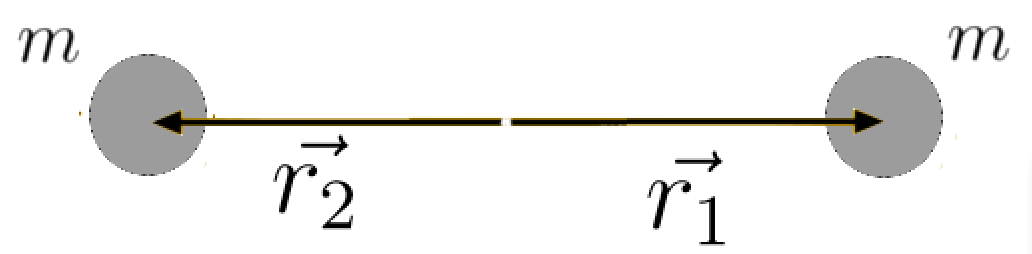
\includegraphics[width=0.7\linewidth]{screenshot001}
		\caption{Posição dos átomos no referencial do centro de massa.}
		\label{fig:fig1}
	\end{figure}

	\question \label{ques:q2}
	Uma vez que conseguimos escrever a energia total do nosso sistema para um potencial genérico, podemos estudar o seu comportamento para um potencial específico. A energia potencial que descreve a interação interatômica é apresentada abaixo
	\begin{equation}\label{eq:Ur}
		U(r) = A\del{1 - \mathrm{e}^{-a(r-b)}}^{2}
	\end{equation}
	onde $ A $, $ a $ e $ b $ são constantes positivas com as dimensões apropriadas. Primeiramente, estudaremos o comportamento do potencial ao redor do mínimo. Para isso, mostre que $ r = r_e = b $ é o mínimo do potencial apresentado em \ref{eq:Ur}.

	\begin{solution}

	\end{solution}

	\question \label{ques:q3}
	Estude agora em que região esse potencial gera uma força atrativa e em qual essa força é repulsiva.
	\begin{parts}
		\part \label{part:q3a} Determine quais são essas regiões.

		\begin{solution}

		\end{solution}

		\part \label{part:q3b} Discuta como o comportamento da força em cada uma dessas regiões está associado ao fato de o mínimo obtido no item anterior ser um ponto de equilíbrio estável.

		\begin{solution}

		\end{solution}
	\end{parts}

	\question \label{ques:q4}
	Conseguimos descrever o comportamento de funções nas proximidades de um certo ponto utilizando a expansão de Taylor. Para uma função $ f(x) $, a expansão de Taylor até a segunda ordem ao redor do ponto $ x_0 $, onde a ordem representa a maior potência de $ x - x_0 $ na expansão, é dada por
	\begin{equation}\label{eq:taylorS}
		f(x)\simeq f(x_0)+\dfrac{f'(x_0)}{1!}(x-x_0)+f\dfrac{f''(x_0)}{2!}(x-x_0)^{2},
	\end{equation}
	onde $ f'(x_0) $ e $ f''(x_0) $ são a primeira e a segunda derivada da função calculadas no ponto $ x_0 $, respectivamente.
	\begin{parts}
		\part \label{part:q4a} Utilize essa expansão para mostrar que o potencial ao redor do ponto $ r_e $ é aproximado por
		\begin{equation}\label{eq:UrApprox}
			U(r) = A\,a^{2}(r-r_e)2.
		\end{equation}

		\begin{solution}

		\end{solution}

		\part \label{part:q4b} Discuta porque é vantajoso utilizarmos a expansão até o termo de segunda ordem ao invés da expansão até o termo de primeira ordem.

		\begin{solution}

		\end{solution}
	\end{parts}

	\question \label{ques:q5}
	Com a aproximação feita no item anterior, escreva:
	\begin{parts}
		\part \label{part:q5a} Qual é a expressão para a energia total do sistema, ou seja, a energia cinética mais a energia potencial próxima ao ponto $ r_e $.

		\begin{solution}

		\end{solution}

		\part \label{part:q5b} Mostre que essa energia é a mesma energia de um oscilador harmônico simples, em relação ao deslocamento relativo $ r - r_e $, e determine a constante elástica associada.

		\begin{solution}

		\end{solution}
	\end{parts}

	\question \label{ques:q6}
	Suponha agora que a velocidade relativa entre os átomos é praticamente zero, a distância entre eles é aproximadamente igual a re e queremos separá-los, ou seja, que a distância entre eles seja aproximadamente infinita. Nesse contexto, responda.

	\begin{parts}
		\part \label{part:q6a} Durante esse processo de separação, o trabalho que a força associada a $ U(r) $ faz é positivo ou negativo?

		\begin{solution}

		\end{solution}

		\part \label{part:q6b} Com base com o que você respondeu no item anterior, o sistema perde ou ganha energia cinética devido a esse trabalho?

		\begin{solution}

		\end{solution}

		\part \label{part:q6c} Como podemos relacionar trabalho realizado com a energia potencial do ponto $ r_e $ e do ponto final?

		\begin{solution}

		\end{solution}

		\part \label{part:q6d} Qual o mínimo de energia que deve ser fornecida ao sistema para que essa separação seja possível? Essa energia é o que chamamos de energia de dissociação $ E_D $.

		\begin{solution}

		\end{solution}
	\end{parts}

	\question \label{ques:q7}
	Tendo em mente do que fizemos nos itens anteriores, faça:
	\begin{parts}
		\part \label{part:q7a} um gráfico de $ U(r) $ deixando claro o ponto que representa $ r_e $ e onde podemos identificar $ E_D $;

		\begin{solution}

		\end{solution}

		\part \label{part:q7b} neste gráfico que você acabou de fazer, identifique uma energia total em que o sistema estaria no estado ligado e uma energia total em que o mesmo estaria no estado não ligado.

		\begin{solution}

		\end{solution}
	\end{parts}

	\extra{Item extra}

	\question \label{ques:q8}
	Para uma molécula de N$_2$ sabemos que $ A = \SI{9,905}{\electronvolt} $, $ a = \SI[per-mode=reciprocal]{2,691e10}{\per\meter} $ e $ b = \SI{1,098e-10}{\meter} $, faça o gráfico do potencial através de algum software (Mathematica, Python, Desmos, etc).

\end{questions}
\end{document}
